\documentclass{article}
    \usepackage{amssymb}
    \usepackage{color}
    \usepackage{listings}
    \usepackage{graphicx}
    \usepackage{subcaption}
    \usepackage{geometry}
    \usepackage{float}
    \geometry{
    a4paper,
    total={170mm,257mm},
    left=20mm,
    top=20mm,
    }

    \setlength{\parindent}{0em}
    \setlength{\parskip}{1em} % length of the spacing
    
    \lstset{ % General setup for the package
        language=Python,
        basicstyle=\small\sffamily,
        numbers=left,
        numberstyle=\tiny,
        frame=tb,
        tabsize=4,
        columns=fixed,
        showstringspaces=false,
        showtabs=false,
        keepspaces,
        commentstyle=\color{red},
        keywordstyle=\color{blue},
        emphstyle=\ttb\color{deepred},    
        stringstyle=\color{deepgreen}
    }
    
    \begin{document}
        \begin{figure}
            \centering
            
\includegraphics[width=0.5\linewidth]{./img/vub.png}
        \end{figure}
        \title{Navigation and Intelligent Vehicles, Lab session # 3 Report}
        \author{Juan Jose Soriano Escobar }
        \maketitle
        \newpage

        \tableofcontents
        \newpage
    
        \begin{appendix}
            \listoffigures
          \end{appendix}
          \newpage
    
    
            \section{Introduction}
            Modelling is an important part of any System or product development that helps to undrestand the model system an holistic point of view and to ensure that all the functionalities and
            stakeholders requirements are cover. One of the most popullar modeling tools nowadays in the software and product development environment is UML.

            UML is ....

            In this report, a Hospital appointment and billing system management are described and modeled in UML as result of the concepts and diagrams learnt in the corse Modellig Languages.

            The description of the model in this report will be splitted by diagram types, covering use case, sequence, activity, state and class diagram.
             
            \newpage         
            \section{Use Case Diagram}
            A use case captures a contract between the stakeholders of a system about its behavior describes the
            system’s behavior under various conditions as it responds to a request from the “primary actor”
            (Delligatti, Steiner, & Soley, 2013).
            \begin{figure}[H]
                \centering 
                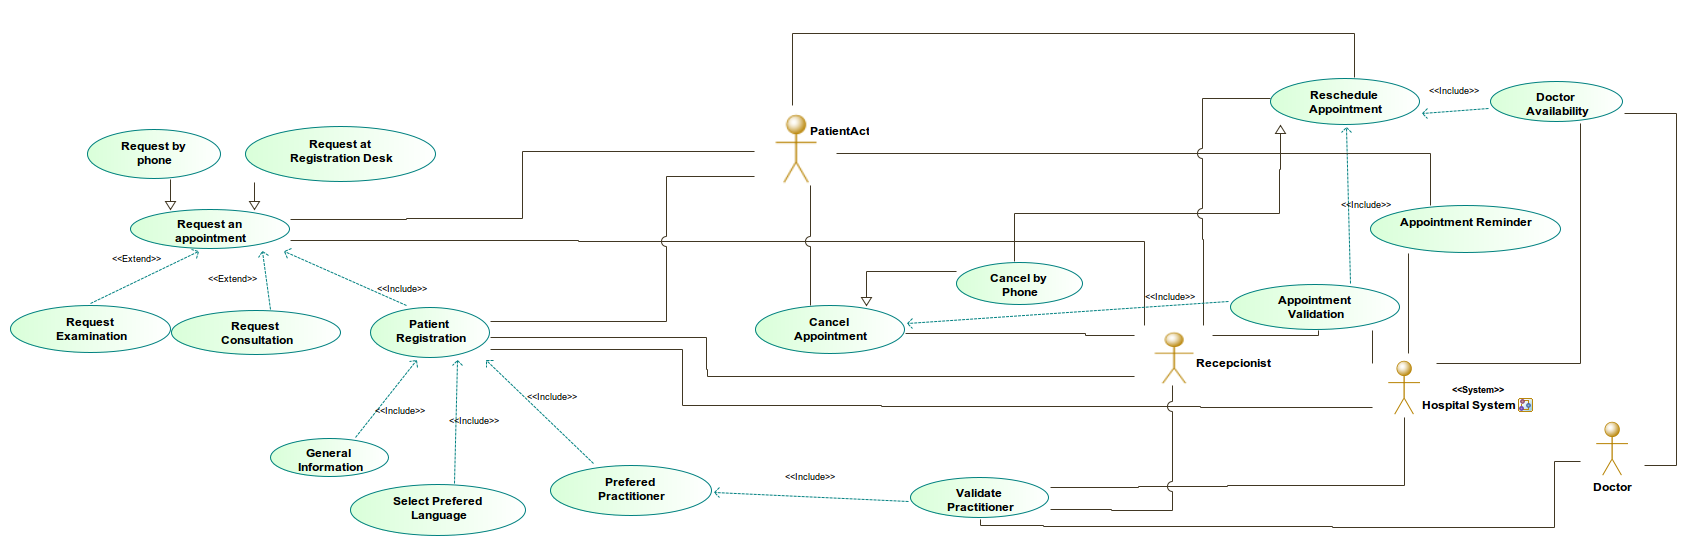
\includegraphics[width=1\linewidth]{./img/appointments.png}
                \setcaptioncitation{self-made}
                \caption{Distributed Computing Implementation.}
                \label{fig:architecture}
            \end{figure}
            \begin{figure}[H]
                \centering 
                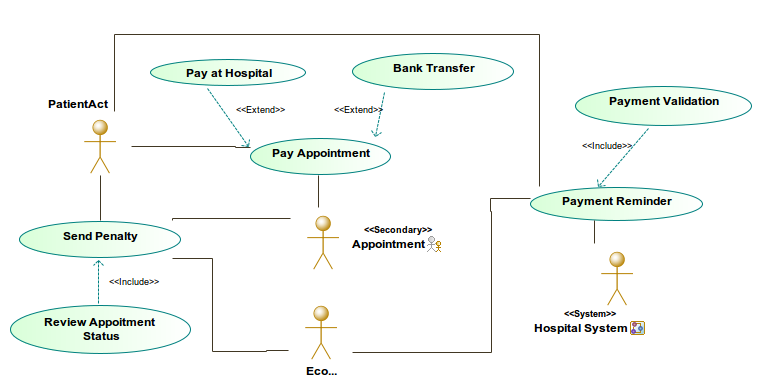
\includegraphics[width=1\linewidth]{./img/payments.png}
                \setcaptioncitation{self-made}
                \caption{Distributed Computing Implementation.}
                \label{fig:architecture}
            \end{figure}
            \begin{figure}[H]
                \centering 
                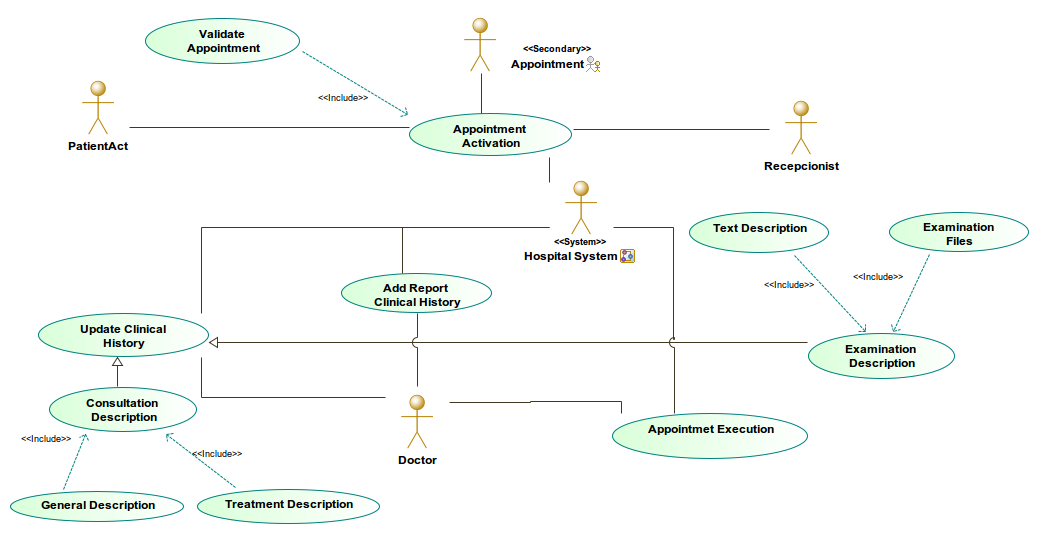
\includegraphics[width=1\linewidth]{./img/cHistories.png}
                \setcaptioncitation{self-made}
                \caption{Distributed Computing Implementation.}
                \label{fig:architecture}
            \end{figure}
            \section{Class Diagram} %reformulate
            Class diagram describes the attributes and operations of a class and also the constraints 
            imposed on the system. The class diagrams are widely used in the modeling of objectoriented 
            systems because they are the only UML diagrams, which can be mapped directly with object-oriented languages.
            \begin{figure}[H]
                \centering 
                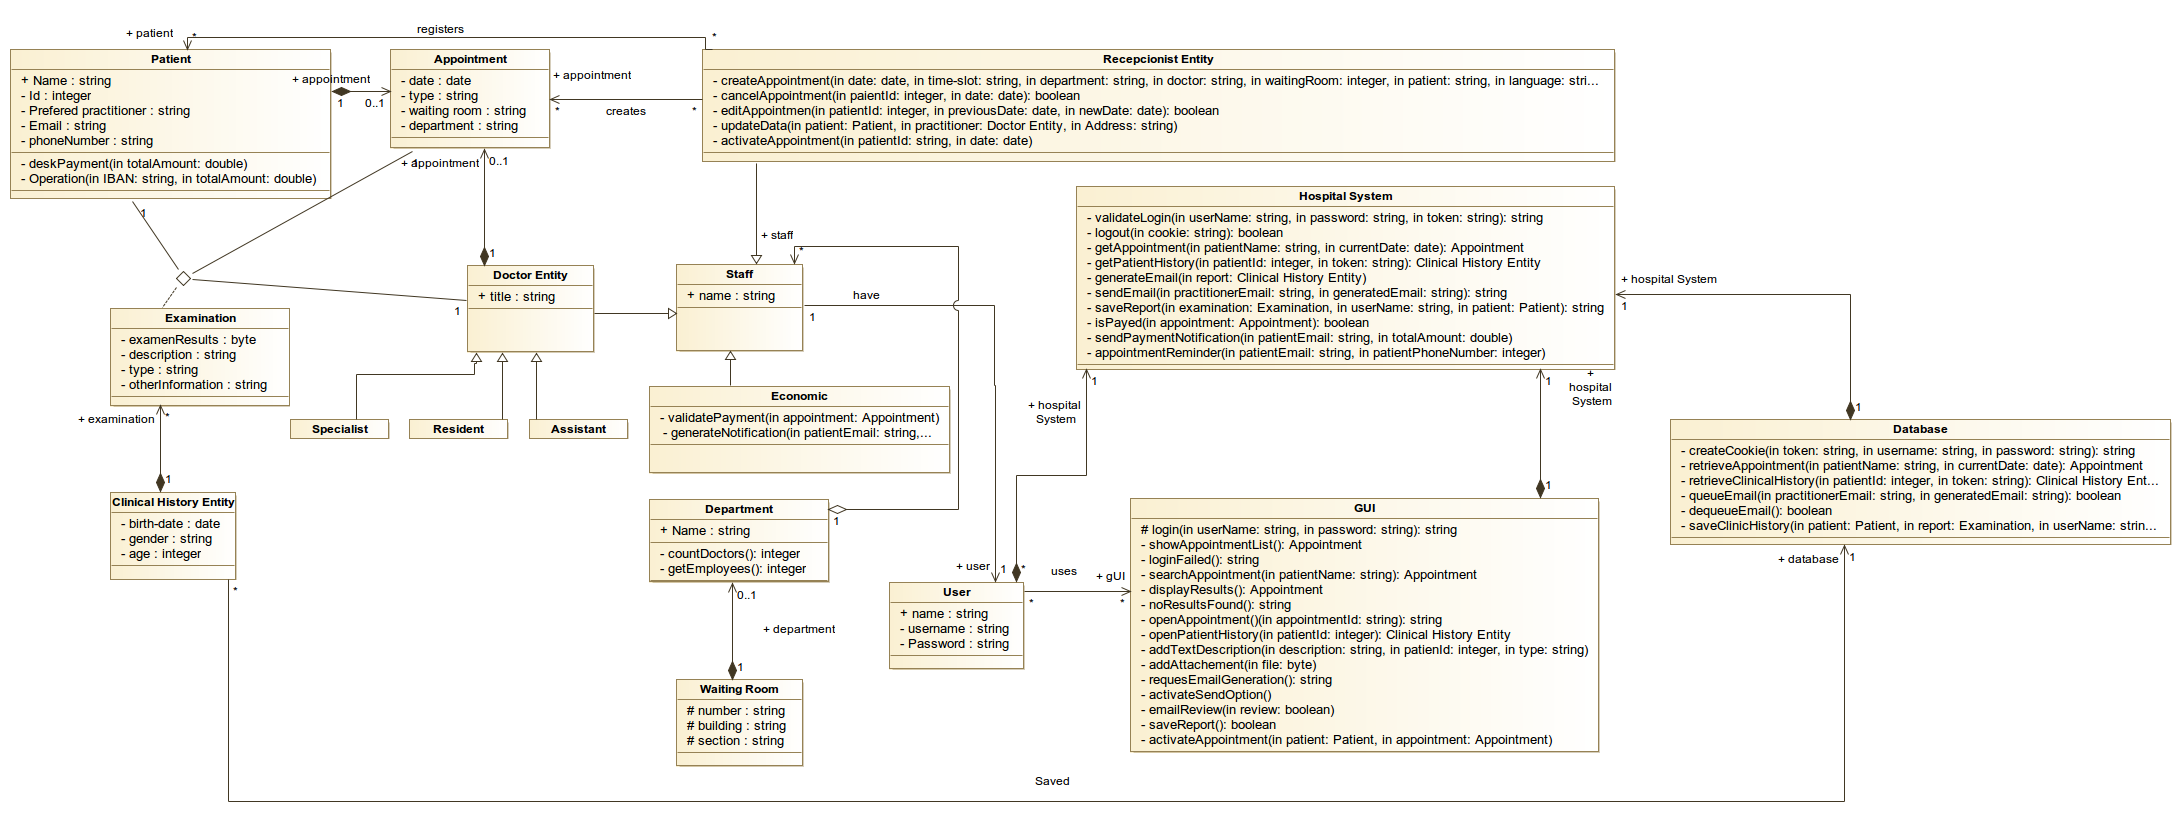
\includegraphics[width=1\linewidth]{./img/class.png}
                \setcaptioncitation{self-made}
                \caption{Distributed Computing Implementation.}
                \label{fig:architecture}
            \end{figure}
            \section{Sequence Diagram}
            Next to the activity diagram is the State Machine Diagram, which is also a behavior
            diagram focus on how a structure within a system changes in response to event
            occurrences over time. It refers to the behavior that begins executing the moment a block
            is instantiated and generally finishes executing when that instance is destroyed
            \begin{figure}[H]
                \centering 
                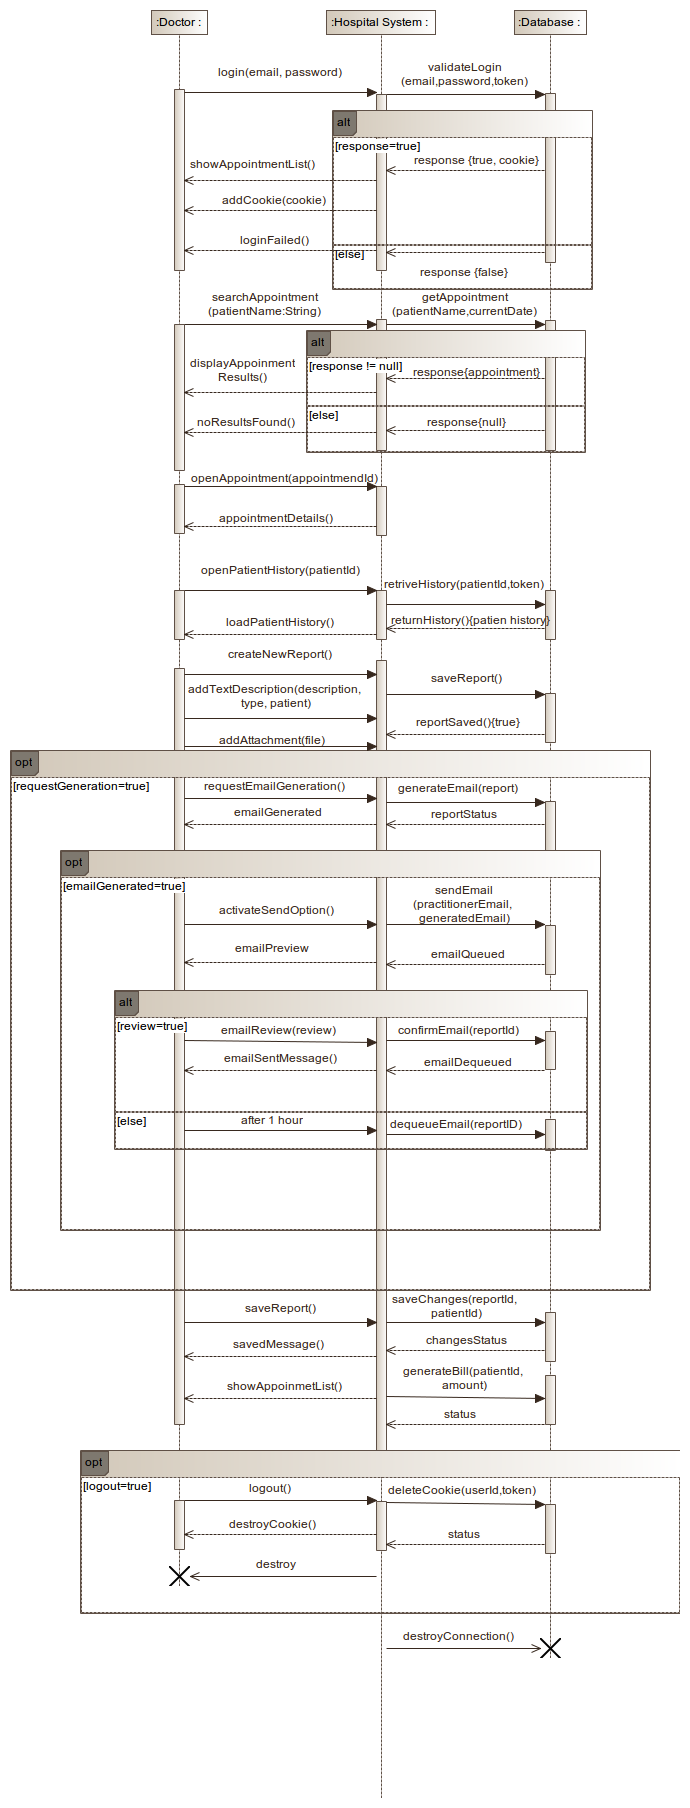
\includegraphics[width=1\linewidth]{./img/seq.png}
                \setcaptioncitation{self-made}
                \caption{Distributed Computing Implementation.}
                \label{fig:architecture}
            \end{figure}
            \section{Activity Case Diagram}
            The activity diagrams are dynamic views of the system that expresses sequence of
            behaviors and event occurrence over time (Delligatti, Steiner, & Soley, 2013). Together
            with the state machine diagram, the system behavior is expressed.
            \begin{figure}[H]
                \centering 
                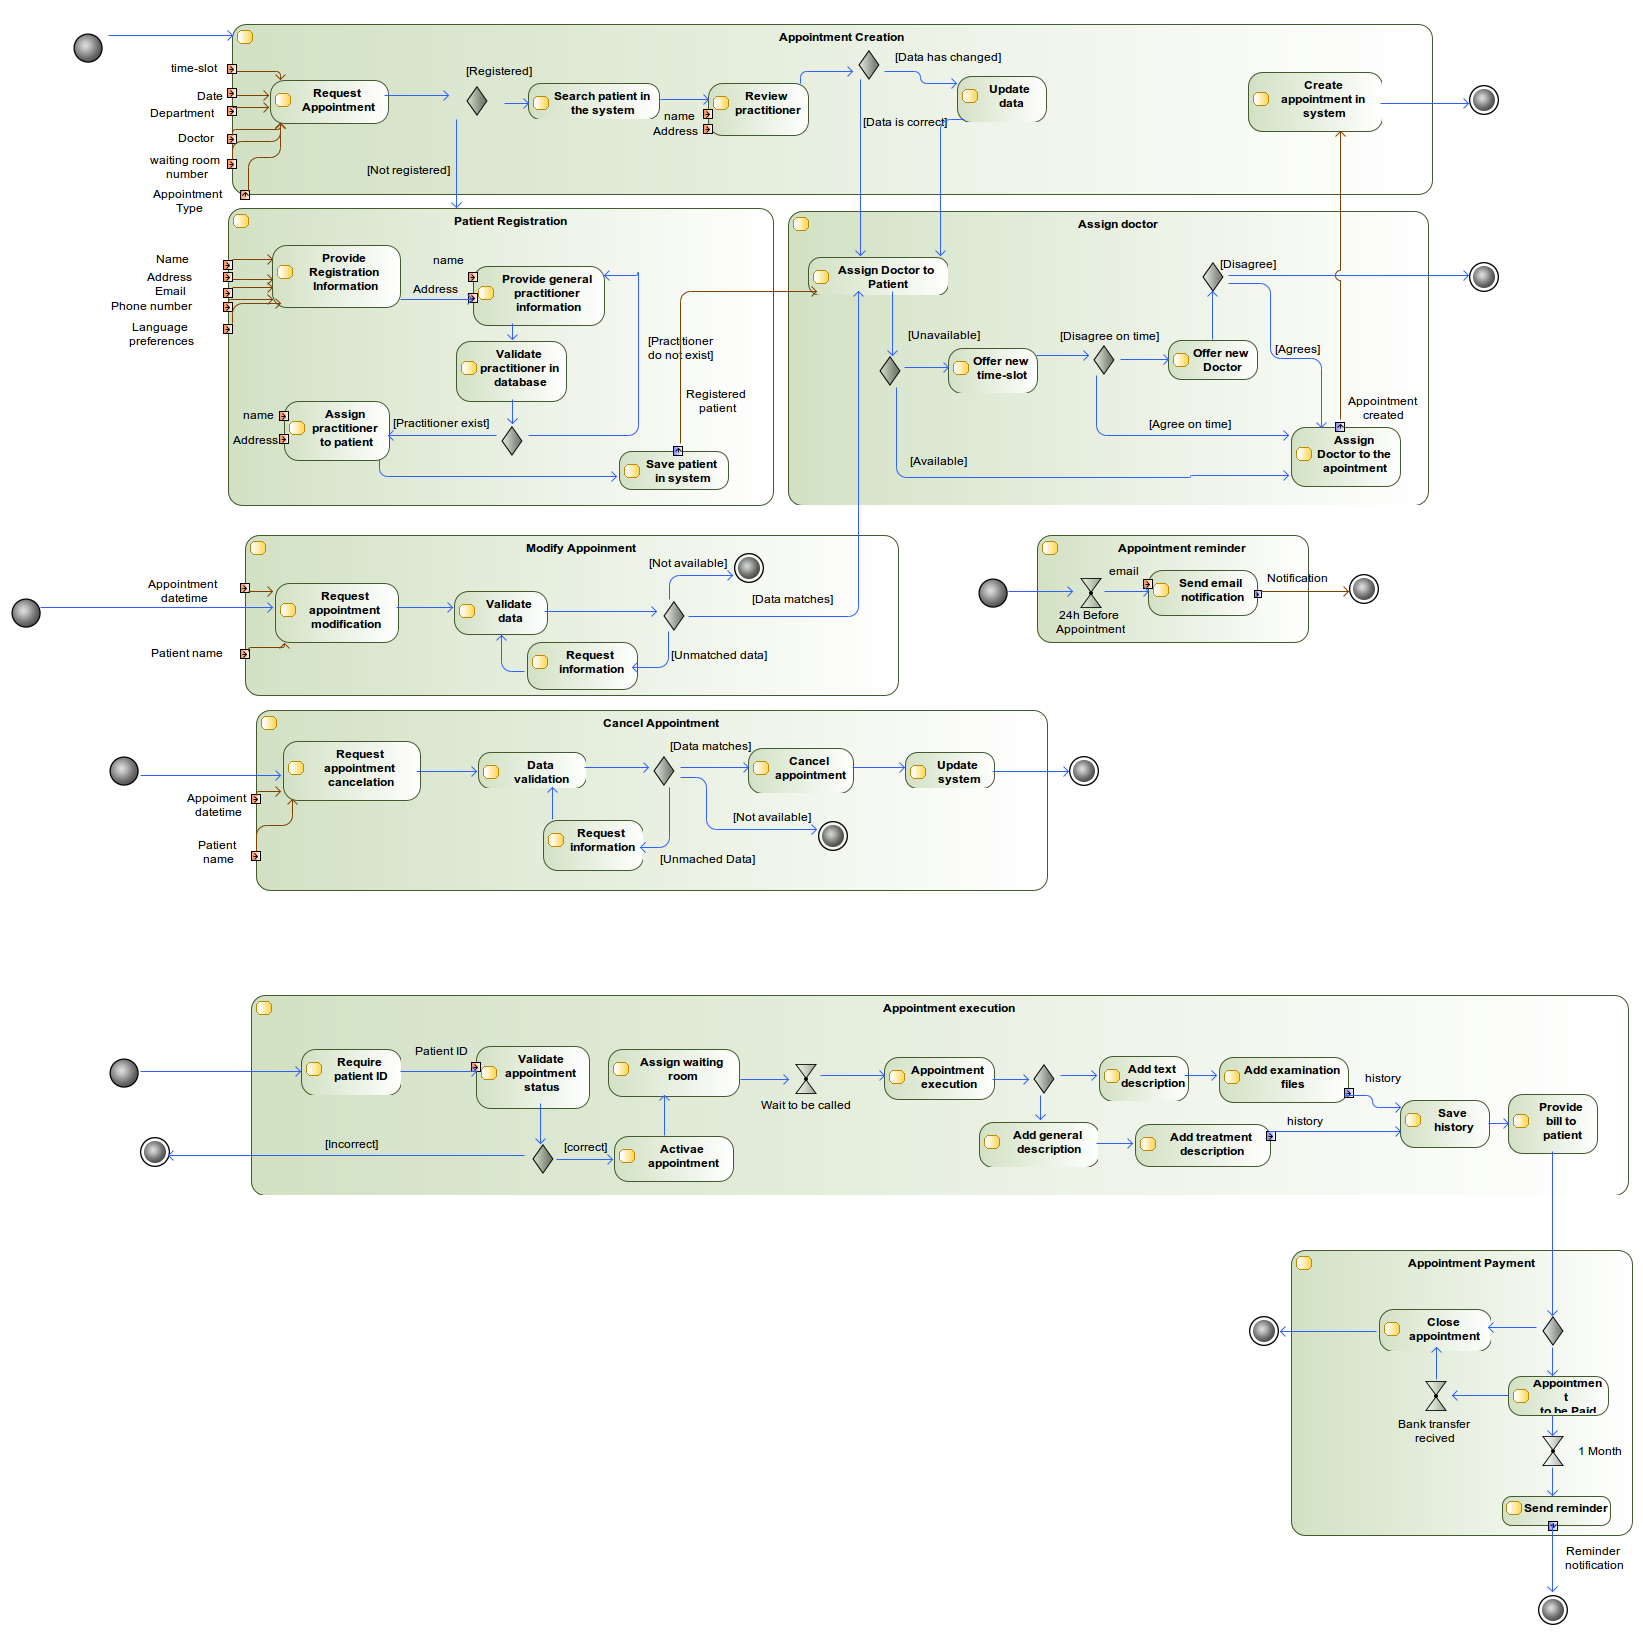
\includegraphics[width=1\linewidth]{./img/Activity.png}
                \setcaptioncitation{self-made}
                \caption{Distributed Computing Implementation.}
                \label{fig:architecture}
            \end{figure}
            \section{State Diagram}
            In this project, we tried to go further with the implementation by combining concepts that we learned in previous courses of the master, such as Web technologies and Databases.  
            We tried to simulate in a "real case" environment, where several devices with different applications or different back-end (e.g. mobile application in Python and web application in Nodejs) are used to collect a specific information and save it in a pre-defined database.
    
            \begin{figure}[H]
                \centering 
                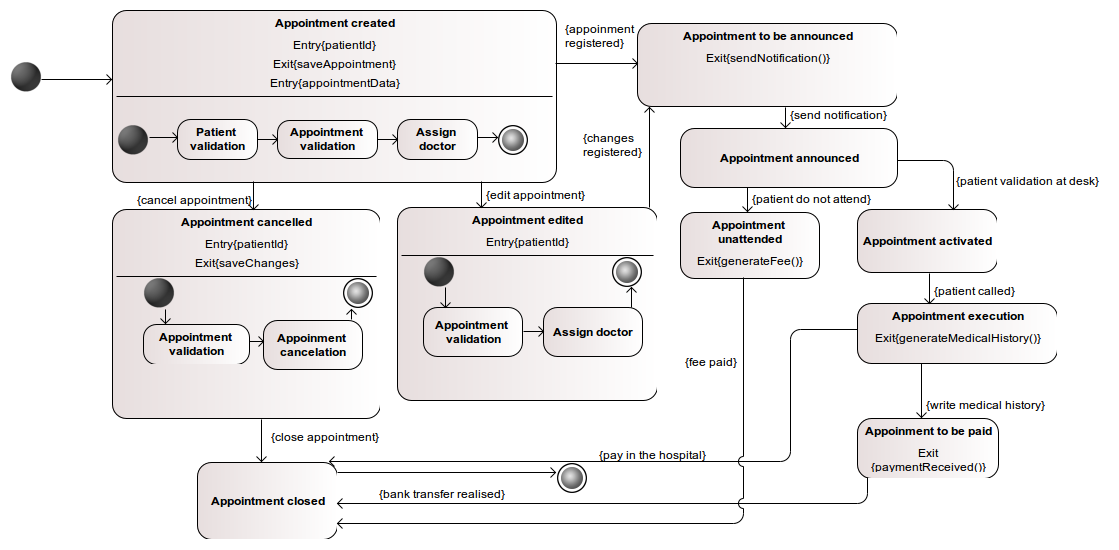
\includegraphics[width=1\linewidth]{./img/state.png}
                \setcaptioncitation{self-made}
                \caption{Distributed Computing Implementation.}
                \label{fig:architecture}
            \end{figure}
    
        
    \end{document}